\section{Pianificazione}
Lo sviluppo del progetto è costruito sulla base delle scadenze riportate nella sottosezione \textsection1.5 ed è suddiviso nelle seguenti fasi:
\begin{itemize}
	\item analisi;
	\item consolidamento dei requisiti
	\item progettazione architetturale;
	\item progettazione di dettaglio e codifica;
	\item validazione e collaudo.
\end{itemize}

\subsection{Analisi}
\textbf{Periodo}: dal 2020-03-10 al 2020-04-13 \\
Questo periodo ha inizio con la formazione dei gruppi e termina con la scadenza per la consegna dei documenti relativi alla \textit{Revisione dei Requisiti}. \\
Le principali attività svolte in questo periodo sono:
\begin{itemize}
	\item \textbf{Strumenti di lavoro}: questa attività consiste nella scelta degli strumenti di lavoro da utilizzare per lo svolgimento del progetto;
	\item \textbf{\NdP{}}: attività nella quale gli Amministratori redigono le \textit{\NdP{}}, documento in cui si specificano tutte le regole, le convenzioni e le tecnologie che i componenti del gruppo adotteranno durante tutto il corso del progetto. Questa attività include una stesura iniziale del documento, comprensiva delle norme e degli standard accordati dal gruppo, il documento verrà poi ampliato in base all'individuazione di sezioni da ampliare;
	\item \textbf{\SdF{}}: attività nella quale gli Analisti redigono lo \textit{\SdF}, documento in cui vengono analizzati i capitolati d'appalto elencando per ciascuno i punti positivi e negativi che li caratterizzano. Inoltre vengono indicate le motivazioni per le quali è stato scelto il capitolato\ped{\textit{G}} C2 denominato \textit{Etherless} e sono stati esclusi i capitolati restanti. \\
	Questa attività è bloccante per l'inizio dell'\textit{\AdR{}};
	\item \textbf{\AdR{}}: attività nella quale gli Analisti redigono l'\textit{\AdR{}}, documento essenziale in cui viene analizzato in maniera approfondita il capitolato\ped{\textit{G}} scelto a seguito dello \textit{\SdF}, individuando le funzionalità e i casi d'uso previsti dal progetto;
	\item \textbf{\PdP{}}: attività nella quale il Responsabile redige il \textit{\PdP}, documento in cui viene presentata la pianificazione del gruppo per lo sviluppo del progetto, un'analisi dei rischi e dei costi e dove vengono indicate le scadenze che il gruppo intende rispettare per la buona riuscita del progetto;
	\item \textbf{\PdQ{}}: attività nella quale gli Analisti redigono il \textit{\PdQ}, documento in cui vengono indicate tutte le strategie di verifica e validazione che il gruppo intende adottare con lo scopo di garantire la qualità di processo e di prodotto\ped{\textit{G}};
	\item \textbf{\Glossario{}}: attività nella quale viene redatto il \textit{\Glossario}, documento nel quale verranno elencati, chiariti ed approfonditi tutti i termini tecnici utilizzati nei documenti con lo scopo di evitare possibili ambiguità;
	\item \textbf{Lettera di Presentazione}: attività nella quale viene redatta la \textit{Lettera di Presentazione} necessaria per la presentazione come fornitore del gruppo.
\end{itemize}
	\subsubsection{Diagramma di Gantt: Analisi}
		\begin{figure}[h]
			\centering
			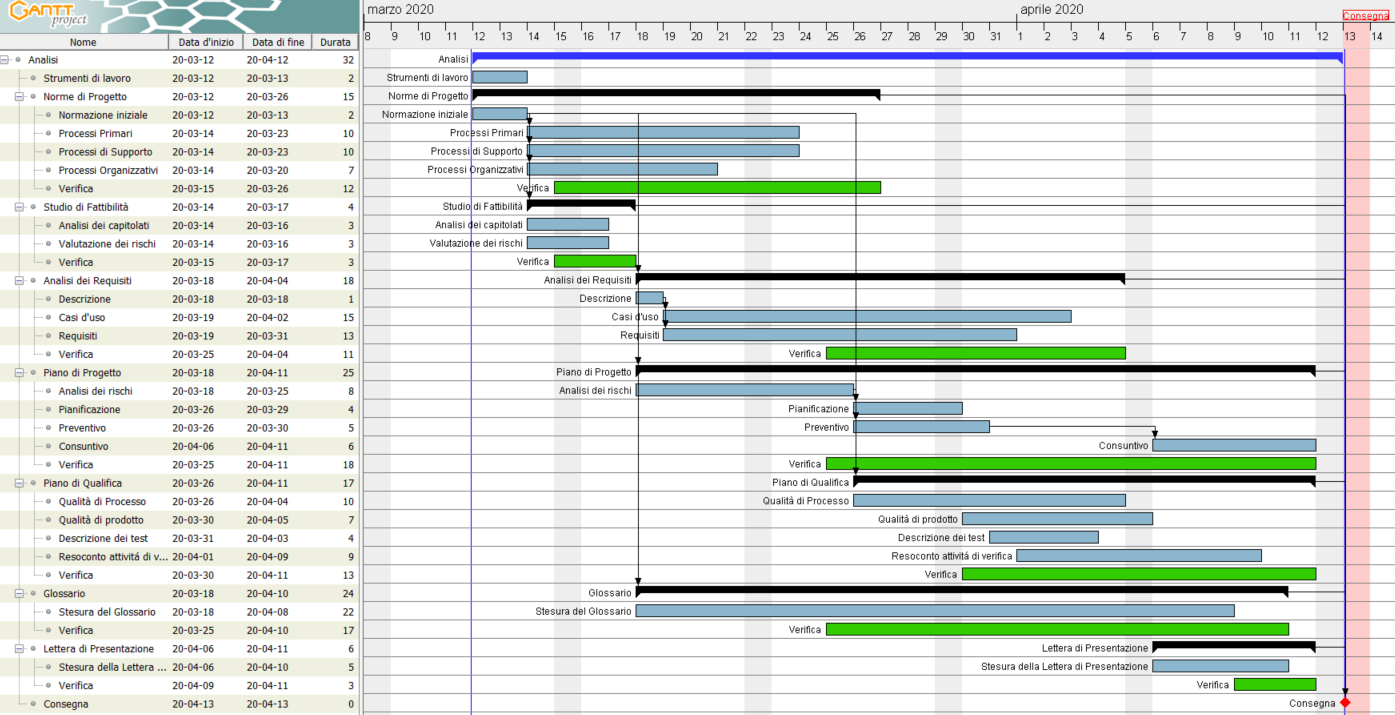
\includegraphics[width=1.1\textwidth]{./res/img/DiagrammiGantt/analisi_gantt.png}
			\caption{Diagramma di Gantt del periodo di Analisi}
		\end{figure}

\subsection{Consolidamento dei Requisiti}
\textbf{Periodo}: dal 2020-04-13 al 2020-04-20 \\
Questo periodo ha inizio dopo il termine del periodo di Analisi e termina il giorno della presentazione della \textit{Revisione dei Requisiti}. \\
\begin{itemize}
	\item \textbf{Incremento e Verifica dei documenti:} in caso di necessità, vengono migliorati e verificati i documenti preparati nel periodo precedente;
	\item \textbf{Consolidamento Analisi dei requisiti}: l'attività principale, prevede un consolidamento e un miglioramento dei requisiti ottenuti concluso il periodo di Analisi e conseguente aggiornamento dell'\textit{\AdR{}};
	\item \textbf{Realizzazione della presentazione:} preparazione del materiale necessario alla presentazione del 2020-04-20.
\end{itemize}
	\subsubsection{Diagramma di Gantt: Consolidamento dei Requisiti}
		\begin{figure}[h]
			\centering
			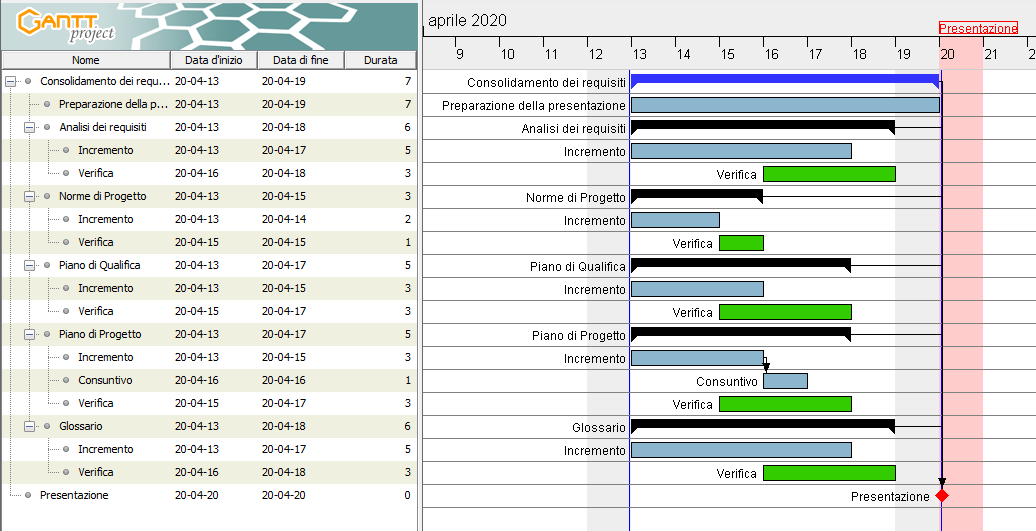
\includegraphics[width=1.1\textwidth]{./res/img/DiagrammiGantt/cons_req_gantt.png}
			\caption{Diagramma di Gantt del periodo di Consolidamento dei Requisiti}
		\end{figure}
\newpage
\subsection{Progettazione Architetturale}
\textbf{Periodo}: dal 2020-04-20 al 2020-05-18 \\
Questo periodo ha inizio al termine del periodo di Consolidamento dei Requisiti e termina alla \textit{Revisione di Progettazione}. \\
Questo periodo porta all'individuazione di una soluzione architetturale che permetta il soddisfacimento dei requisiti individuati.
\begin{itemize}
	\item \textbf{Incremento e verifica}: come prima cosa, analizzando l'esito della \textit{Revisione dei Requisiti} vengono svolte attività di incremento e verifica sui vari documenti redatti, dove necessario. \\
	L'incremento dell'\textit{\AdR{} 1.0.0} è il più importante perchè va completato prima di poter proseguire con il resto delle attività;
	\item \textbf{Technology Baseline}: viene redatta la documentazione di supporto, contenente la descrizione delle tecnologie individuate e il tracciamento della relazione tra le componenti e i requisiti che vanno a soddisfare. Viene anche codificato il \textbf{PoC (Proof of Concept)} come dimostrazione del funzionamento dell'architettura individuata;
	\item \textbf{Glossario}: attività che prevede un miglioramento del \textit{\Glossario{} 1.0.0} aggiungendo nuovi termini oppure raffinando le definizioni di termini già presenti.
\end{itemize}
	\subsubsection{Incrementi}
		\subsubsubsection{Descrizione}
			\begin{itemize}
				\item \textbf{1° Incremento:} integrazione dei documenti a seguito delle conoscenze acquisite nei periodi precedenti;
				\item \textbf{2° Incremento:} implementazione della componente Etherless-smart;
				\item \textbf{3° Incremento:} implementazione della componenete Etherless-cli; \\
				Comandi da implementare per il PoC, legati ai requisiti che soddisfano:
					\rowcolors{2}{lightRowColor}{darkRowColor}
					\begin{longtable}{
						>{\centering}p{0.25\textwidth}
						>{\centering}p{0.20\textwidth} }

						\coloredTableHead
						\textbf{\color{white}Comando} &
						\textbf{\color{white}Requisiti}
						\tabularnewline
						\endhead

						\hline \multicolumn{2}{c}{\textit{Continua nella prossima pagina}} \\
						\endfoot
						\hline
						\endlastfoot
						signup & R1F3\\ R1F3.1 \\ R1F3.1.1 \\ R1F3.1.2 \\ R1F3.1.3\tabularnewline
						login & R1F4 \\ R1F4.1 \\ R1F4.1.1 \\ R1F4.1.2\tabularnewline
						logout & R1F5\tabularnewline
						run & R1F9 \\ R1F9.1 \\ R1F9.2 \\ R1F9.3\tabularnewline
						\rowcolor{white}\caption{Tracciamento comandi-requisiti soddisfatti}	\\

					\end{longtable}
				\item \textbf{4° Incremento:} implementazione della componente Etherless-server;
				\item \textbf{5° Incremento:} integrazione delle componenti sviluppate;
				\item \textbf{6° Incremento:} correzione della documentazione a seguito della correzione della RR e preparazione in vista della \TB{};
				\item \textbf{7° Incremento:} ulteriori aggiornamenti della documentazione, con passaggio alla versione 2.0.0:
				\begin{itemize}
					\item consuntivo di periodo nel \PdP{};
					\item aggiornamento \NdP{} e \PdQ{};
					\item eventuali aggiornamenti riguardanti il \Glossario{}.
				\end{itemize}
				\item \textbf{8° Incremento:} preparazione della presentazione per la RP.
			\end{itemize}
		\subsubsubsection{Scadenze}
			\begin{itemize}
				\item \textbf{1° Incremento:} entro 2020-04-22;
				\item \textbf{2° Incremento:} entro 2020-04-24;
				\item \textbf{3° Incremento:} entro 2020-04-26;
				\item \textbf{4° Incremento:} entro 2020-04-27;
				\item \textbf{5° Incremento:} entro 2020-04-28; % 29???
				\item \textbf{6° Incremento:} entro 2020-05-04;
				\item \textbf{7° Incremento:} entro 2020-05-11;
				\item \textbf{8° Incremento:} entro 2020-05-18.
			\end{itemize}

	\subsubsection{Diagramma di Gantt: Progettazione Architetturale}
		\begin{figure}[h]
			\centering
			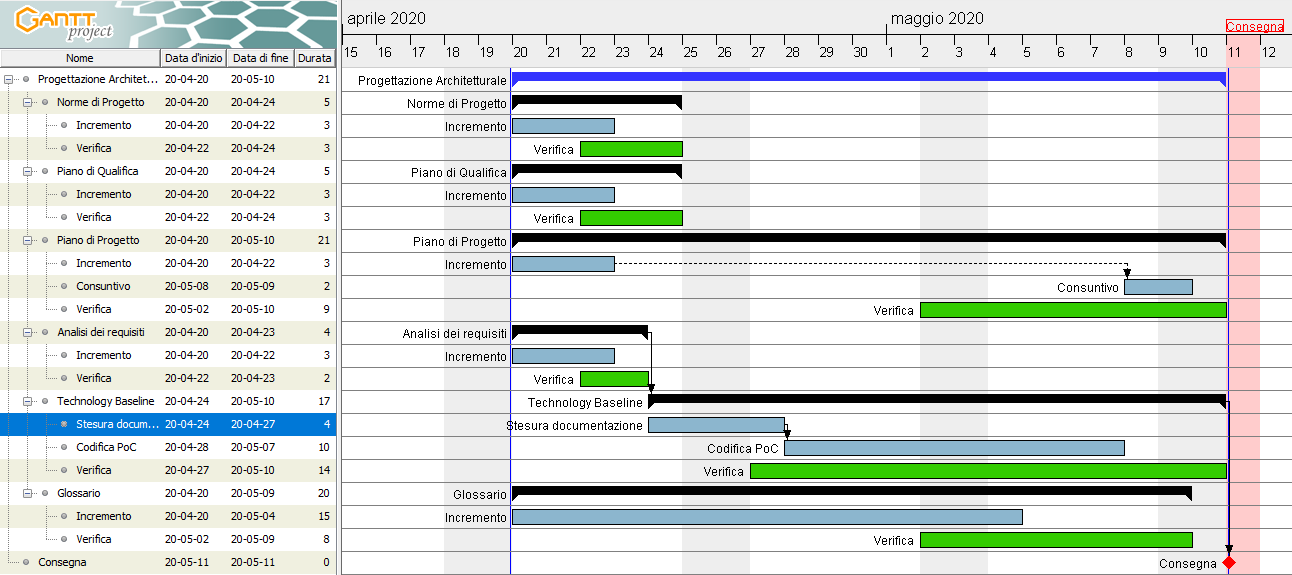
\includegraphics[width=1.1\textwidth]{./res/img/DiagrammiGantt/prog_arch_gantt.png}
			\caption{Diagramma di Gantt del periodo di Progettazione Architetturale}
		\end{figure}
\newpage
\subsection{Progettazione di Dettaglio e Codifica}
\textbf{Periodo}: dal 2020-05-11 al 2020-06-18 \\
Questo periodo ha inizio dopo il termine del periodo di Progettazione Architetturale e termina con la \textit{Revisione di Qualifica}. \\
Le principali attività svolte in questo periodo sono:
\begin{itemize}
	\item \textbf{Incremento e verifica}: come prima cosa, analizzando l'esito della \textit{Revisione dei Progettazione} vengono svolte attività di incremento e verifica sui vari documenti redatti;
	\item \textbf{Product Baseline}: progettazione dettagliata a basso livello delle componenti del prodotto\ped{\textit{G}}, coerente con quanto individuato nella \TB{}:
	\begin{itemize}
		\item \textbf{Allegato Tecnico}: stesura del documento di \textit{Allegato Tecnico 1.0.0}, di supporto alla progettazione di dettaglio;
		\item \textbf{Codifica}: attività nelle quali viene prodotto e verificato il codice.
	\end{itemize}
	\item \textbf{User Manual} (manuale utente): attività nella quale viene redatto lo \textit{User Manual 1.0.0} contenente le informazioni su come funziona e su come si utilizza il prodotto\ped{\textit{G}};
	\item \textbf{Glossario}: attività che prevede un miglioramento del \textit{Glossario 2.0.0} aggiungendo nuovi termini oppure raffinando le definizioni di termini già presenti.
\end{itemize}
	\subsubsection{Incrementi}
		\subsubsection{Descrizione}
			\begin{itemize}
				\item \textbf{1° Incremento:} correzione e integrazione dei documenti a seguito delle conoscenze acquisite nei periodi precedenti;
				\item \textbf{2° Incremento:} progettazione dei 3 moduli che compongono il sistema e stesura dell'\textit{Allegato Tecnico 1.0.0};
				\item \textbf{3° Incremento:} sviluppo di Etherless-smart;
				\item \textbf{4° Incremento:} realizzazione delle componenti Etherless-CLI e Etherless-server (comprensivi di test di unitá e di integrazione);\\
				Comandi da implementare, legati ai requisiti che la loro implementazione va a soddisfare:

						\rowcolors{2}{lightRowColor}{darkRowColor}
						\begin{longtable}{
							>{\centering}p{0.25\textwidth}
							>{\centering}p{0.20\textwidth} }

							\coloredTableHead
							\textbf{\color{white}Comando} &
							\textbf{\color{white}Requisiti}
							\tabularnewline
							\endhead

							\hline \multicolumn{2}{c}{\textit{Continua nella prossima pagina}} \\
							\endfoot
							\hline
							\endlastfoot

							% Contenuto della tabella
							% Ruolo & Ore & Costo\\
							signup & R1F3\\ R1F3.1 \\ R1F3.1.1 \\ R1F3.1.2 \\ R1F3.1.3\tabularnewline
							login & R1F4 \\ R1F4.1 \\ R1F4.1.1 \\ R1F4.1.2 \\ R1F4.1.3\tabularnewline
							logout & R1F5\tabularnewline
							info & R1F7 \\ R1F7.1 \\ R1F7.2 \tabularnewline
							run & R1F9 \\ R1F9.1 \\ R1F9.1.1 \\ R1F9.2 \\ R1F9.2.1 \\ R1F9.2.2 \\ R1F9.3 \\ R1F9.4 \tabularnewline
							list & R1F10 \\ R1F10.1 \\ R1F10.2 \\ R1F10.3 \\ R1F10.4 \tabularnewline
							deploy & R1F11 \\ R1F11.1 \\ R1F11.1.2 \\ R1F11.2 \\ R1F11.2.1 \\ R1F11.2.2 \\ R1F11.4\tabularnewline
							edit & R1F12 \\ R1F12.1 \\ R1F12.1.1 \\ R1F12.1.2 \\ R1F12.2 \\ R1F12.2.1 \\ R1F12.3 \\ R1F12.3.1 \\ R1F12.3.2\tabularnewline
							delete & R1F14 \\ R1F14.1 \\ R1F14.1.1 \\ R1F14.1.2\tabularnewline

							\rowcolor{white}\caption{Tracciamento comandi-requisiti soddisfatti}	\\

						\end{longtable}

				\item \textbf{5° Incremento:} stesura documenti:
				\begin{itemize}
					\item stesura dello \textit{User Manual 1.0.0}.
				\end{itemize}
				Ulteriori aggiornamenti della documentazione, con passaggio alla versione 3.0.0:% (consuntivo di periodo PdP e user manual)
					\begin{itemize}
						\item consuntivo di periodo nel \PdP{};
						\item aggiornamento dell'\textit{Allegato Tecnico};
						\item eventuali aggiornamenti riguardanti il \Glossario{}.
					\end{itemize}
				\item \textbf{6° Incremento:} preparazione della presentazione per la RQ.
			\end{itemize}
		\subsubsection{Scadenze}
			\begin{itemize}
				\item \textbf{1° Incremento:} entro 2020-05-20;
				\item \textbf{2° Incremento:} entro 2020-05-24;
				\item \textbf{3° Incremento:} entro 2020-05-26;
				\item \textbf{4° Incremento:} entro 2020-06-05;
				\item \textbf{5° Incremento:} entro 2020-06-11;
				\item \textbf{6° Incremento:} entro 2020-06-18.
			\end{itemize}
	\subsubsection{Diagramma di Gantt: Progettazione di Dettaglio e Codifica}
		\begin{figure}[h]
			\centering
			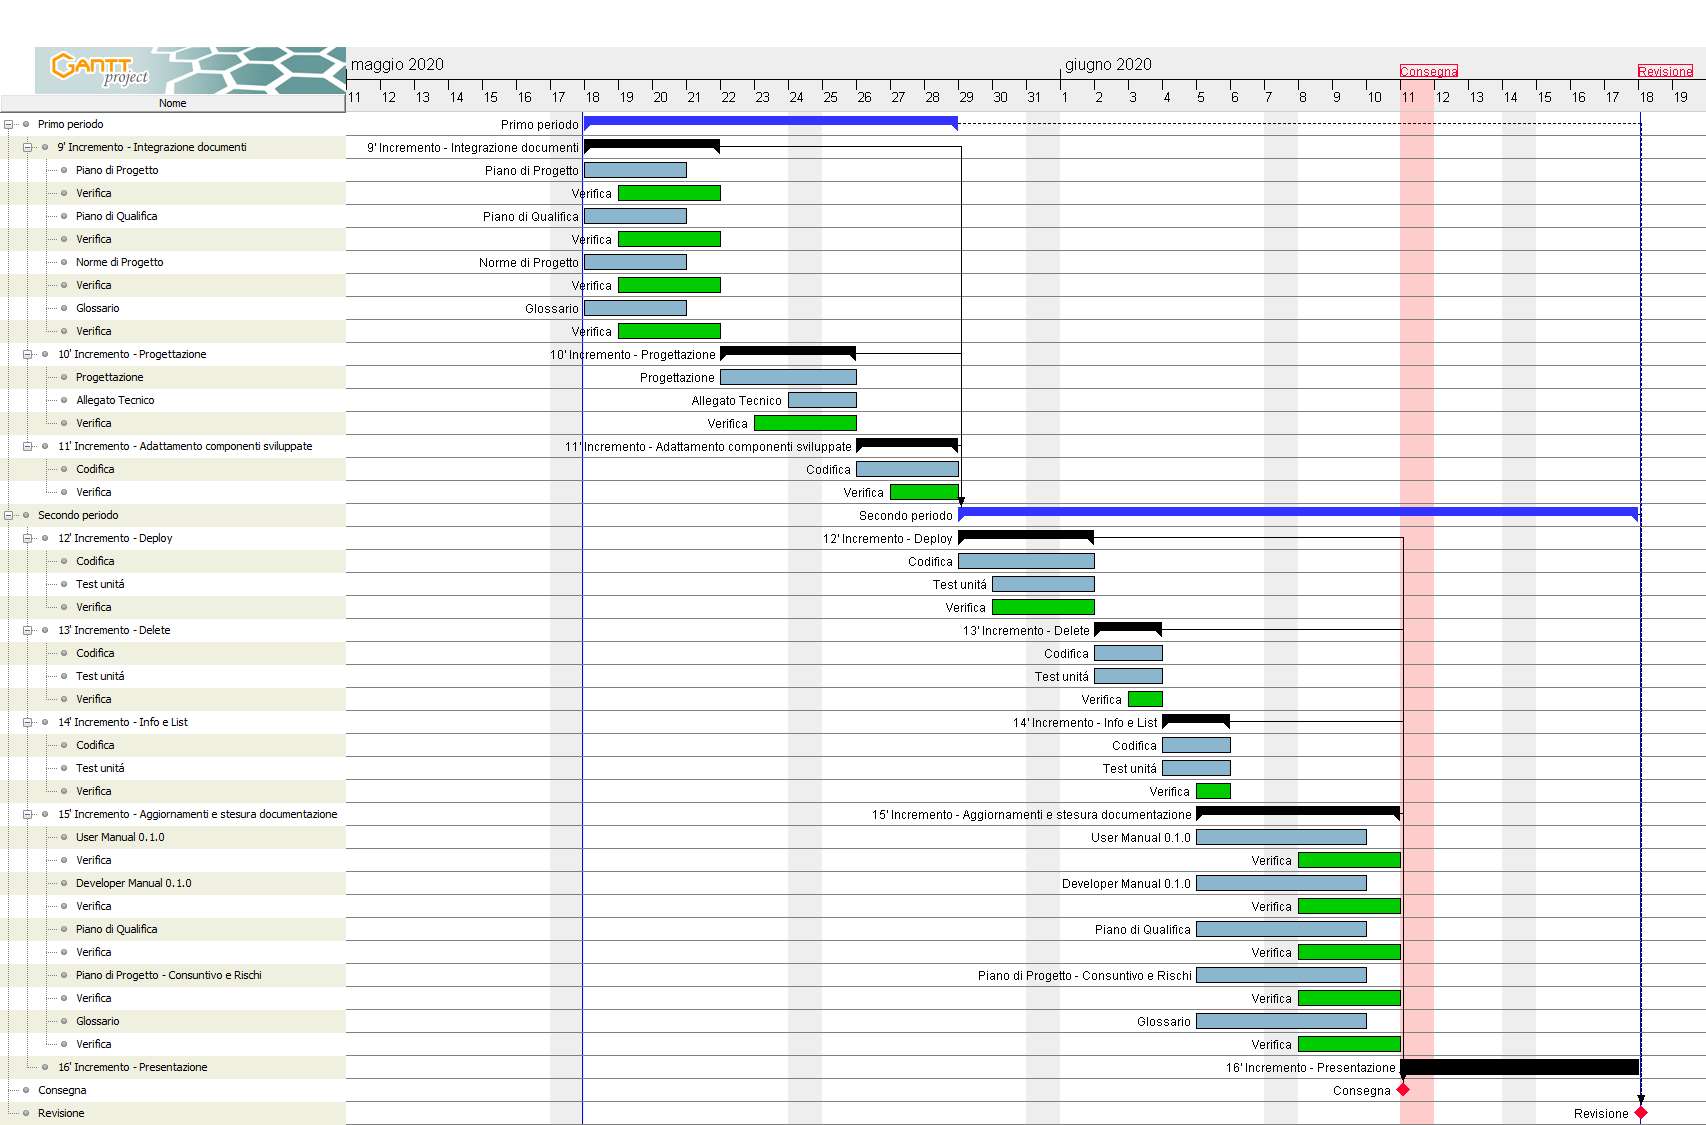
\includegraphics[width=1.1\textwidth]{./res/img/DiagrammiGantt/prog_dett_gantt.png}
			\caption{Diagramma di Gantt del periodo di Progettazione di Dettaglio e Codifica}
		\end{figure}
\newpage
\subsection{Validazione e Collaudo}
\textbf{Periodo}: dal 2020-06-11 al 2020-07-20 \\
Questo periodo ha inizio dopo il termine del periodo di Progettazione di Dettaglio e Codifica, e termina con la \textit{Revisione di Accettazione}. \\
Le principali attività svolte in questo periodo sono:
\begin{itemize}
	\item \textbf{Incremento e verifica}: come prima cosa, analizzando l'esito della \textit{Revisione dei Qualifica} vengono svolte attività di incremento e verifica sui vari documenti redatti;
	\item \textbf{Validazione e Collaudo}: attività nella quale vengono eseguiti test e, se necessario, vengono apportati dei miglioramenti al prodotto\ped{\textit{G}} per poter assicurare il soddisfacimento dei requisiti e dei vincoli qualitativi;
	\item \textbf{User Manual}: attività nella quale viene migliorato lo \textit{User Manual 1.0.0};
	\item \textbf{Manuale Sviluppatore}: attività nella quale viene redatto il \textit{Manuale Sviluppatore 1.0.0}, il quale contiene le informazioni utili al mantenimento del prodotto\ped{\textit{G}};
	\item \textbf{Glossario}: attività che prevede un miglioramento del \textit{Glossario 3.0.0} aggiungendo nuovi termini oppure raffinando le definizioni di termini già presenti.
\end{itemize}
	\subsubsection{Incrementi}
		\subsubsubsection{Descrizione}
			\begin{itemize}
				\item \textbf{1° Incremento:} correzione e integrazione dei documenti a seguito delle conoscenze acquisite nei periodi precedenti e dalla correzione della RQ;
				\item \textbf{2° Incremento:} implementazione dei requisiti mancanti, ovvero quelli desiderabili e opzionali;\\
				Comandi da implementare, legati a requisiti desiderabili e opzionali:
					\begin{itemize}
						\item \textbf{init};
						\item \textbf{help:} legato a UC1 e UC2;
						\item \textbf{whoami:} legato allo UC9;
						\item \textbf{search:} legato allo UC11;
						\item \textbf{history:} legato allo UC16.
					\end{itemize}
				\item \textbf{3° Incremento:} implementazione dei test di sistema ed eventuali correzioni necessarie;
				\item \textbf{4° Incremento:} aggiornamento dei documenti e stesura del \textit{Manuale dello Sviluppatore 1.0.0};
				\item \textbf{5° Incremento:} preparazione della presentazione per la RA.
			\end{itemize}
		\subsubsubsection{Scadenze}
			\begin{itemize}
				\item \textbf{1° Incremento:} entro 2020-06-26;
				\item \textbf{2° Incremento:} entro 2020-07-02;
				\item \textbf{3° Incremento:} entro 2020-07-08;
				\item \textbf{4° Incremento:} entro 2020-07-13;
				\item \textbf{5° Incremento:} entro 2020-07-20.
			\end{itemize}
	\subsubsection{Diagramma di Gantt: Validazione e Collaudo}
		\begin{figure}[h]
			\centering
			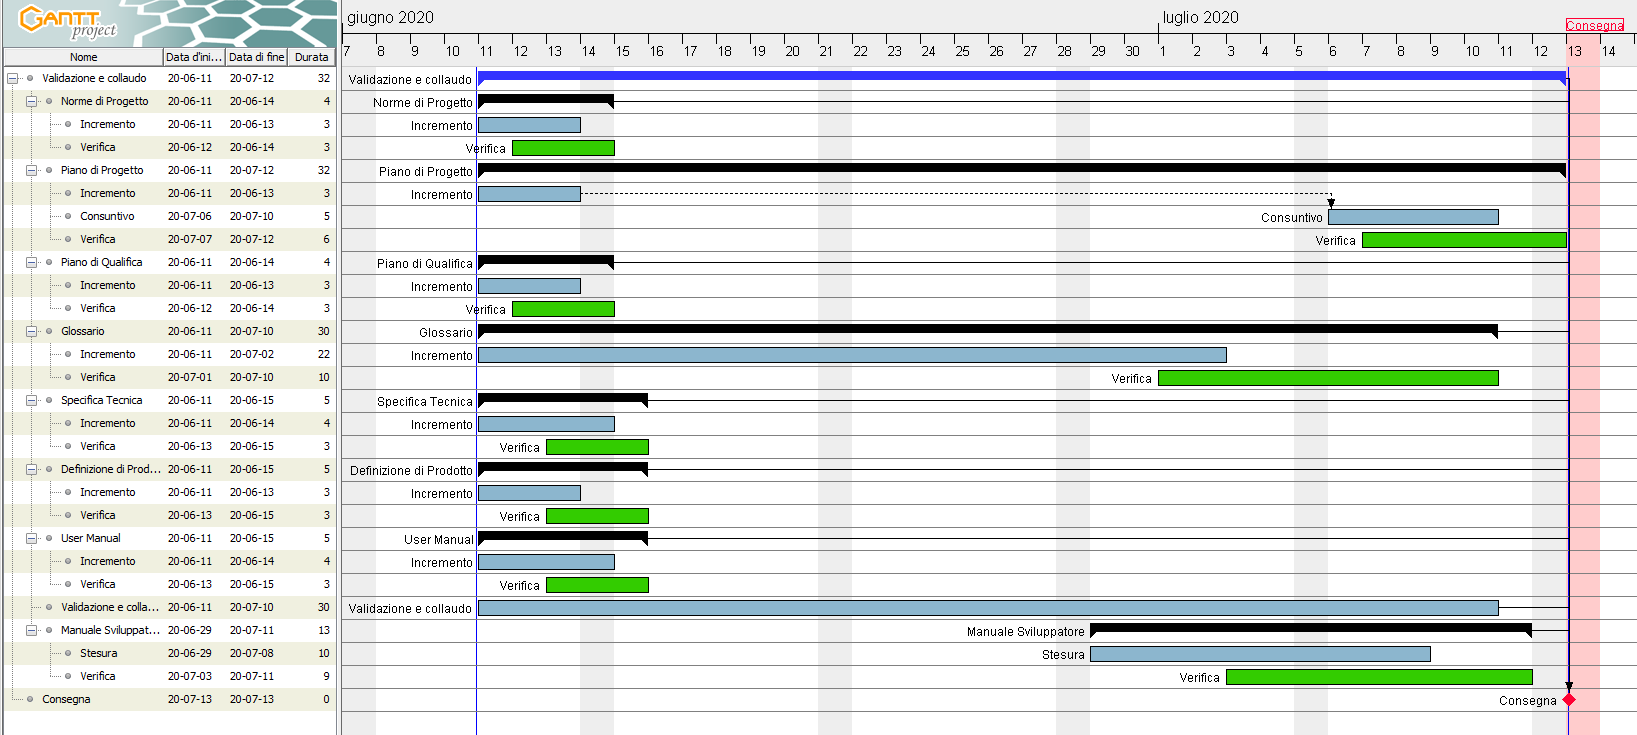
\includegraphics[width=1.1\textwidth]{./res/img/DiagrammiGantt/validaz_gantt.png}
			\caption{Diagramma di Gantt del periodo di Validazione e Collaudo}
		\end{figure}
